\documentclass[11pt]{article}
\usepackage[margin=1in]{geometry}
\usepackage{amsmath,amssymb,amsthm}
\newtheorem{proposition}{Proposition}
\newtheorem*{remark}{Remark}
\usepackage{booktabs}
\usepackage{array}
\usepackage{enumitem}
\usepackage{caption}
\usepackage{tikz}
\usetikzlibrary{positioning,arrows.meta,fit}
\usepackage[colorlinks=true,linkcolor=black,urlcolor=blue,citecolor=black]{hyperref}
\usepackage{titlesec}

\titleformat{\section}{\normalfont\large\bfseries}{\thesection}{0.6em}{}
\titleformat{\subsection}{\normalfont\normalsize\bfseries}{\thesubsection}{0.6em}{}
\setlist{itemsep=2pt,parsep=0pt,topsep=4pt}
\captionsetup{font=small,labelfont=bf}

\newcommand{\CC}{\mathcal{C}}
\newcommand{\NN}{\mathcal{N}}
\newcommand{\PP}{\mathcal{P}}
\newcommand{\Lcal}{\mathcal{L}}
\newcommand{\Xcal}{\mathcal{X}}
\newcommand{\Acal}{\mathcal{A}}
\newcommand{\Ecal}{\mathcal{E}}
\newcommand{\Tcal}{\mathcal{T}}
\newcommand{\1}{\mathbb{1}}
\newcommand{\node}[2]{\textsf{#1\,:\,#2}}
\newcommand{\Wt}{\widetilde{W}}

\title{\bfseries Operationalizing a Coherence-Based Framework\\ for Ideology in Discourse\\[4pt]
\large V3.2: sparse additive rates, faceted ideologies, one co-occurrence channel\\ \large with a timescale, a shared association layer, and structural coherence}
\author{Working notes}
\date{\today}

\begin{document}
\maketitle

\begin{abstract}
\noindent An ideology is a pair $(\eta_k, W_k)$: a sparse deviation of log expression rates from a background, over typed response-level nodes, and a nonnegative excess co-occurrence network over pairs that do not skip rungs of the ladder $V\!-\!A\!-\!B\!-\!R$ (intra-type links admitted). The codebook maps each concept to a single stance-bearing node, and each ideology carries a small number of \emph{facets}: sub-profiles over the same network, the granularity at which specialists engage. Actors are mixed memberships over (ideology, facet) pairs plus a background coordinate and a breadth scalar---no free actor-by-concept deviations---so actor variation is rank-restricted to the span of the facets, and the identification of the association layer does not compete with an actor shrinkage scale. Alignment is a regression on actor identity metadata. Expressions are conditionally independent Poisson draws from the actor's rates: there is no within-expression co-occurrence model, and the rate layer is fully generative. Co-occurrence is instead handled by an estimating equation, not a likelihood: pair counts derived from the data at an analyst-set timescale $\delta$---a kernel over an actor's unit pairs, with same-expression co-occurrence and co-occurrence-within-actor-ever as the two endpoints---are scored against a Poisson working model, and $W_k$ is the excess of kernel-weighted pair counts over what the actor's own margins and a \emph{shared association layer} $W^{(0)}$ predict, routed to ideologies by alignment. The shared layer implements the distinction between ideology and culture or commonsense: shared meanings that allow interaction across groups live in the background rates and $W^{(0)}$; ideology is what covaries with alignment, because it operates where power is contested between groups. Structural coherence---concepts relating more, or more strongly, within an ideology than across its boundary---is measured per ideology against a permutation null, and optionally encouraged by a support-gated sparsity prior; logical coherence is the incompatibility caps. The expression layer is a structural topic model with SAGE components over concepts rather than words; the association layer---one edge set read at a chosen timescale---is the departure, since topic models have no pairwise interaction term. Theory enters as priors and caps. All numerical results are TBD.
\end{abstract}

\section{Two kinds of contrast, and a ladder}\label{sec:contrast}

Two organizing ideas carry through, and one structural commitment.

\paragraph{Exclusion contrast.} Ideologies can differ by which \emph{level} of an attitude they occupy. Colorblindness holds \node{race}{peripheral}; intersectionality holds \node{race}{central}. Levels of one concept are mutually exclusive, so the two are separated by non-adjacency, with no negative relation needed.

In the present operationalization the codebook resolves stance into the concept definitions themselves: each concept carries a single node, so $\NN=\CC$ and the node index $u$ and concept index $c$ coincide. Exclusion contrast is then expressed through incompatible concept pairs (C3) rather than levels of one concept; the level machinery is retained in the definitions for codebooks that resolve it.

\paragraph{Relational contrast.} Ideologies can share a node and differ in what it connects to. Intersectionality and racial nationalism both hold \node{race}{central}; one links it to structural racism and redistribution, the other to natural hierarchy and separation. A shared node with ideology-specific edges cannot live in one pooled graph (Section~\ref{sec:single}); it requires a separate network per ideology.

\paragraph{Ideology, culture, commonsense.} Ideologies are not universally shared because they operate in spaces where power is contested between groups (van Dijk 1998); culture and commonsense are shared meanings that allow interaction \emph{across} groups. The model implements the distinction as an estimand rather than an assumption: shared meaning lives in facets available to every actor (background rates, temporal offsets, and a shared association layer $W^{(0)}$), and ideology is whatever expression and association covary with group alignment. How much of a discourse is culture and how much is contested is then an output (Section~\ref{sec:inference}).

\paragraph{The type ladder.} Concepts are of four types. Relations run within a type and between adjacent types---what the ladder forbids is \emph{rung-skipping}:
\begin{center}
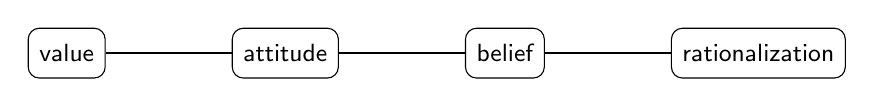
\begin{tikzpicture}[node distance=16mm,
  every node/.style={draw,rounded corners,font=\small\sffamily,inner sep=4pt,minimum height=18pt}]
  \node (v) {value};
  \node (a) [right=of v] {attitude};
  \node (b) [right=of a] {belief};
  \node (r) [right=of b] {rationalization};
  \draw[-,thick] (v)--(a); \draw[-,thick] (a)--(b); \draw[-,thick] (b)--(r);
\end{tikzpicture}
\end{center}
Values ground attitudes; attitudes are supported by beliefs; beliefs are defended by rationalizations; and concepts of one type can be linked among themselves (belief--belief entailments, attitude constellations, value systems). An ideology's network is layered in the weaker, cross-rung sense: any path from a value to a rationalization passes through an attitude and a belief, so the middle layers mediate between distant rungs by construction, while structure within a rung is unconstrained beyond sparsity.

\section{The model: a generative rate layer, an estimating pair channel}\label{sec:generative}

\paragraph{Fixed inputs.} Concept set $\CC$ with type map $T:\CC\to\{V,A,B,R\}$; nodes $\NN=\CC$ (one stance-bearing node per concept; $u$ and $c$ used interchangeably); facet counts $F_k$ per ideology, with $F_0=1$; allowed pairs
\[
  \PP=\big\{(u,u'):\ u\ne u',\ \{T(u),T(u')\}\notin\big\{\{V,B\},\{V,R\},\{A,R\}\big\}\big\},
\]
i.e.\ same-type and adjacent-type pairs, excluding rung-skipping pairs; actor metadata $m_a$; unit timestamps $t(d)$; a co-occurrence kernel $K_\delta$ with timescale $\delta$; theory sets $\Acal^\pm_k,\Ecal_k,\Xcal,\Tcal^{\text{fix}}$; hyperparameters $\lambda_{\text{sp}},\omega,\alpha,\bar\pi,\sigma_\mu^2,\sigma_\beta^2,\sigma_\xi^2,\sigma_m^2$. The extraction layer supplies $x_{d,u}\in[0,1]$ per unit, treated as expected counts; the extractor judges nodes independently within a unit.

\subsection*{Background}
\begin{itemize}
  \item For each node $u$: set $m_u=\log(\text{corpus rate of }u)$, fixed.
  \item For each time period $t$ and concept $c$: draw the temporal offset $m_{t,c}\sim\mathcal{N}(0,\sigma_m^2)$, applied to all levels of $c$. This is the news cycle: what the world is discussing at $t$, shared across actors, so that event-driven expression is not read as ideology or as actor disposition.
\end{itemize}

\subsection*{Shared association layer}
\begin{itemize}
  \item For each pair $(u,u')\in\PP$: draw $W^{(0)}_{uu'}\sim\text{Exp}(\lambda_{\text{sp}})$, zero off $\PP$ and on same-concept pairs. This is commonsense association: pairings every speaker makes regardless of alignment (schemas, scripts, topical conventions). It is estimated from all actors; without it, the ideology networks silently absorb cultural association and overstate how much structure is ideological.
\end{itemize}

\subsection*{Alignment regression}
\begin{itemize}
  \item For each ideology $k$ and metadata dimension $j$: draw $\beta_{k,j}\sim\mathcal{N}(0,\sigma_\beta^2)$.
\end{itemize}

\subsection*{Ideologies ($k=1,\dots,M$)}
\begin{itemize}
  \item \textbf{Profile.} For each node $u$:
  \begin{itemize}
    \item Draw a variance $\tau^{(I)}_{k,u}\sim\text{Jeffreys}$ (Exponential if a proper prior is wanted).
    \item Draw the sparse deviation $\eta_{k,u}\sim\mathcal{N}\big(\mu^{\text{C1}}_{k,u},\ \tau^{(I)}_{k,u}\big)$, with $\mu^{\text{C1}}_{k,u}=+\alpha$ for $u\in\Acal^+_k$, $-\alpha$ for $u\in\Acal^-_k$, else $0$ (C1).
  \end{itemize}
  Subject to (C3): for every incompatible set $S$, $\sum_{u\in S}e^{m_u+\eta_{k,u}}\le\bar\pi$. The sparsity is substantive: $\eta_{k,u}=0$ is ``no position on $u$''---an ideology takes positions on few nodes, and the scale mixture makes silence the default rather than a budgeted resource. There is no separate background component: the background ideology is the all-zeros deviation.
  \item \textbf{Network.} For each pair $(u,u')\in\PP$: draw $W_{k,uu'}\sim\text{Exp}(\lambda_{\text{sp}})$, shifted so $W_{k,uu'}\ge\omega$ on $\Ecal_k$ (C2). Set $W_{k,uu'}=0$ off $\PP$ (rung-skipping pairs; C5) and on same-concept pairs (C3 structural).
\end{itemize}

\subsection*{Actors ($a=1,\dots,A$)}
\begin{itemize}
  \item Draw soft membership over (ideology, facet) pairs, including the background coordinate:
  \[
    \theta_a=\mathrm{softmax}\big(\underbrace{\beta_k^\top m_a}_{\text{ideology logit}}+\underbrace{\gamma_{a,kf}}_{\text{facet logit}}\big),\qquad
    \gamma_{a,\cdot}\sim\mathcal{N}(0,\sigma_\gamma^2 I),
  \]
  with a point mass on ideology $\bar k_a$ (facets free) for $a\in\Tcal^{\text{fix}}$ (C4). Identity metadata informs \emph{which ideology}; the facet an actor works within it is an actor-level draw. $\vartheta_{a,k}=\sum_f\theta_{a,kf}$ denotes the ideology-level membership; $\theta_{a,0}$, the background coordinate, is the fraction of the actor's speech that is unideological, and it is where off-profile chatter lands instead of clutter or a junk component.
  \item Draw breadth $\mu_a\sim\mathcal{N}(0,\sigma_\mu^2)$.
  \item Set the actor's node rates, additively in log space:
  \[
    \log\eta_{a,u,t}\;=\;\underbrace{m_u+m_{t,u}}_{\text{background}}\;+\;\underbrace{\textstyle\sum_{k,f}\theta_{a,kf}\,\eta_{k,f,u}}_{\text{ideology and facet}}\;+\;\underbrace{\mu_a}_{\text{breadth}}.
  \]
  There are no free actor-by-concept deviations: a specialist is an actor concentrated on one facet, and actor variation is rank-restricted to the span of the facet profiles plus a scalar. A specialist's silence on the rest of the ideology's platform is therefore modeled---it is the facet's silence---without granting actors saturated freedom that would compete with $W$ for between-actor covariation (Section~\ref{sec:build}).
\end{itemize}

\subsection*{Expression}
For each unit $d$, by actor $a=a(d)$ at time $t=t(d)$:
\begin{itemize}
  \item For each node $u$: draw $x_{d,u}\sim\text{Poisson}\big(\eta_{a,u,t}\big)$.
\end{itemize}
Expressions are a sparse set of the actor's facet-composed concepts: conditionally independent draws from the actor's rates. \emph{There is no within-expression co-occurrence model.} At corpus densities the Poisson and a Bernoulli presence model are numerically close; the Poisson is used because the additive log-rate composes with it exactly and every estimation block is a Poisson GLM.

\subsection*{The pair channel: an estimating equation at timescale $\delta$}
For each actor $a$ and pair $(u,u')\in\PP$, the kernel-weighted pair count over the actor's units,
\[
  A^{(\delta)}_{a,uu'}\;=\;\sum_{d,d'}K_\delta\big(t(d)-t(d')\big)\,x_{d,u}\,x_{d',u'},
\]
is drawn as
\[
  A^{(\delta)}_{a,uu'}\;\sim\;\text{Poisson}\Big(N^{(\delta)}_a\;\eta_{a,u}\,\eta_{a,u'}\;e^{\Omega_{a,uu'}}\Big),
  \qquad \Omega_{a,uu'}=W^{(0)}_{uu'}+\textstyle\sum_k\vartheta_{a,k}W_{k,uu'},
  \qquad N^{(\delta)}_a=\sum_{d,d'}K_\delta\big(t(d)-t(d')\big),
\]
using time-averaged rates $\eta_{a,u}$ in the exposure. The timescale is the analyst's variable:
\begin{itemize}
  \item $K_\delta=\1[d=d']$: co-occurrence means \emph{within the same expression}.
  \item $K_\delta\equiv1$: co-occurrence \emph{within an actor, ever}, is equivalent evidence.
  \item Between: decay at scale $\delta$ (e.g.\ $K_\delta=e^{-|t-t'|/\delta}$), interpolating the two assumptions.
\end{itemize}
$W^{(0)}$ absorbs pairing excess common to all actors; $W_k$ is the log excess beyond margins \emph{and} shared association, routed to ideologies by the ideology-level membership $\vartheta_{a,k}$ (facets share their ideology's network): being loud on two concepts is not evidence of an edge, pairing them beyond one's own loudness is evidence of association, and pairing them beyond what everyone does is evidence of ideology. Identification follows the same logic as the rate layer: the shared layer is estimated from all actors, the ideology layers only from excess that covaries with alignment.

\paragraph{How $W$ learns, and what $\delta$ selects.} The gradient on an edge is
\[
  \frac{\partial\log L}{\partial W_{k,uu'}}=\sum_a\vartheta_{a,k}\Big(A^{(\delta)}_{a,uu'}-N^{(\delta)}_a\,\eta_{a,u}\eta_{a,u'}\,e^{\Omega_{a,uu'}}\Big),
\]
and identically for $W^{(0)}$ with the weight $\vartheta_{a,k}$ replaced by $1$.
\[
\]
At small $\delta$, excess is temporal clumping within (or near) single expressions. As $\delta\to\infty$, a within-actor identity binds: the total pair count is determined, up to noise, by the actor's margins,
\[
  A^{(\infty)}_{a,uu'}=n_{a,u}n_{a,u'}-\textstyle\sum_d x_{d,u}x_{d,u'},
\]
so per-actor excess vanishes and $W$ is identified \emph{across} actors: joint elevation of $u$ and $u'$ among $k$'s adherents, beyond what their facet memberships predict, must be carried by the shared edge. Because actor variation is rank-restricted to the facet span (no saturated per-actor deviations), this identification is clean at every $F_k$ short of saturation---the channel hands estimation smoothly from within-actor clumping to between-actor covariation as $\delta$ grows, and $W_k(\delta)$ reported as a curve locates the timescale at which each edge lives. The residual coupling is with the facet count: as $F_k$ grows, facets can absorb covariation the way free deviations did (Section~\ref{sec:build}).

\paragraph{Status of the pair channel.} The pair counts $A^{(\delta)}$ are computed from $x$, and the expression block generates $x$ as conditionally independent given rates---so under the model as written, $A^{(\delta)}$ is determined by $x$ and carries no excess for $W$ to generate. There is no joint distribution over $(x,A^{(\delta)})$ consistent with both blocks, and the document does not claim one. The pair channel is an \emph{estimating equation}: the same dataset is scored twice, once through its margins (a true likelihood) and once through a derived pair statistic against a Poisson working model whose canonical parameter is $\Omega$. This is the standard pseudo-likelihood position for interaction models, adopted because the coherent alternative (Section~\ref{sec:extensions}) is materially heavier. Practical consequences: point estimation is unproblematic; standard errors on $W$ require the composite-likelihood (sandwich) correction, with double-counting growing in $\delta$; comparisons across $\delta$ are made on the excess scale, not raw likelihood; and ``the objective'' (Section~\ref{sec:objective}) is a sum of estimating functions, not a posterior.

\begin{remark}[Unsigned edges lose nothing]
Under a codebook that resolves levels (not the present one): for binary concepts written in level indicators $u^+ + u^- = 1$, any signed coupling $-\omega\,b_ib_j$ equals, up to an additive constant, an attractive coupling of strength $2|\omega|$ between same-level nodes ($\omega>0$) or opposite-level nodes ($\omega<0$); generally, the exclusion identity $\sum_\ell u_{i\ell}=1$ lets any pairwise potential be shifted nonnegative without changing the distribution. Unsigned $W\ge0$ over response levels therefore loses no generality relative to signed edges over concepts, conditional on expression; presence itself is carried by the rate layer.
\end{remark}


\subsection*{Model at a glance}

\begin{center}
\small
\setlength{\tabcolsep}{4pt}\begin{tabular}{@{}lllp{0.27\textwidth}p{0.30\textwidth}@{}}
\toprule
Symbol & Indexed by & Kind & Prior / source & Role \\
\midrule
\multicolumn{5}{@{}l}{\emph{Fixed structure}}\\
$T(c)$ & concept & fixed & codebook & type map $\CC\to\{V,A,B,R\}$ \\
$\NN,\ \PP$ & --- & fixed & derived from $T$, levels & nodes; allowed (non-rung-skipping) pairs \\
$\Acal^\pm_k,\Ecal_k,\Xcal,\Tcal^{\text{fix}}$ & ideology & fixed & theory files & anchors, links, incompatible sets, labeled actors \\
$K_\delta,\ \delta$ & --- & analyst & swept & co-occurrence kernel and timescale \\
$m_u$ & node & fixed & corpus rate & background log-rate \\
\addlinespace
\multicolumn{5}{@{}l}{\emph{Observed}}\\
$m_a$ & actor & observed & data & identity metadata \\
$x_{d,u}$ & unit, node & observed & extractor & expression (expected counts) \\
$t(d),\ a(d)$ & unit & observed & data & timestamp, author \\
$A^{(\delta)}_{a,uu'}$ & actor, pair & derived & from $x$, $K_\delta$ & kernel-weighted pair counts \\
\addlinespace
\multicolumn{5}{@{}l}{\emph{Latent: shared facets (culture)}}\\
$m_{t,c}$ & period, concept & latent & $\mathcal{N}(0,\sigma_m^2)$ & temporal background (news cycle) \\
$W^{(0)}_{uu'}$ & pair $\in\PP$ & latent & $\text{Exp}(\lambda_{\text{sp}})$ & shared association layer \\
\addlinespace
\multicolumn{5}{@{}l}{\emph{Latent: ideologies ($k=1,\dots,M$)}}\\
$F_k$ & ideology & analyst & holdout (V7) & facet count; $F_0=1$ \\
$\eta_{k,f,u}$ & ideology, facet, node & latent & SAGE: $\mathcal{N}(\mu^{\text{C1}}_{k,u},\tau^{(I)}_{k,f,u})$ & sparse facet profile; C1 shifts (per $k$), C3 caps \\
$\tau^{(I)}_{k,f,u}$ & ideology, facet, node & latent & Jeffreys & profile sparsity scale \\
$W_{k,uu'}$ & ideology, pair & latent & $\text{Exp}(\lambda_{k,uu'})$, $\ge\omega$ on $\Ecal_k$ & excess association; C2 support, C5 zeros, C6 gate \\
\addlinespace
\multicolumn{5}{@{}l}{\emph{Latent: actors ($a=1,\dots,A$)}}\\
$\beta_{k,j}$ & ideology, feature & latent & $\mathcal{N}(0,\sigma_\beta^2)$ & identity$\to$alignment regression (C4) \\
$\gamma_{a,kf}$ & actor, (ideology, facet) & latent & $\mathcal{N}(0,\sigma_\gamma^2)$ & facet logits \\
$\theta_{a,kf},\ \vartheta_{a,k}$ & actor & derived & softmax; $\sum_f\theta_{a,kf}$ & membership; ideology margin \\
$\theta_{a,0}$ & actor & derived & (coordinate of $\theta_a$) & unideological share of speech \\
$\mu_a$ & actor & latent & $\mathcal{N}(0,\sigma_\mu^2)$ & breadth / verbosity \\
\addlinespace
\multicolumn{5}{@{}l}{\emph{Derived quantities}}\\
$\eta_{a,u,t}$ & actor, node, period & derived & $\exp(m_u{+}m_{t,u}$ ${+}\sum_{k,f}\theta_{a,kf}\eta_{k,f,u}{+}\mu_a)$ & actor node rate \\
$\Omega_{a,uu'}$ & actor, pair & derived & $W^{(0)}_{uu'}+\sum_k\theta_{a,k}W_{k,uu'}$ & composed association \\
$S_k,\ C_k$ & ideology & derived & $\{u:\max_f\eta_{k,f,u}>0\}$; C6 & support; coherence ratio \\
\midrule
\multicolumn{5}{@{}l}{Hyperparameters: $\alpha,\bar\pi,\omega,\lambda_{\text{sp}},\lambda_{\text{in}},\lambda_{\text{out}},\sigma_m^2,\sigma_\beta^2,\sigma_\gamma^2,\sigma_\mu^2$.}\\
\bottomrule
\end{tabular}
\end{center}

\begin{figure}[h]
\centering
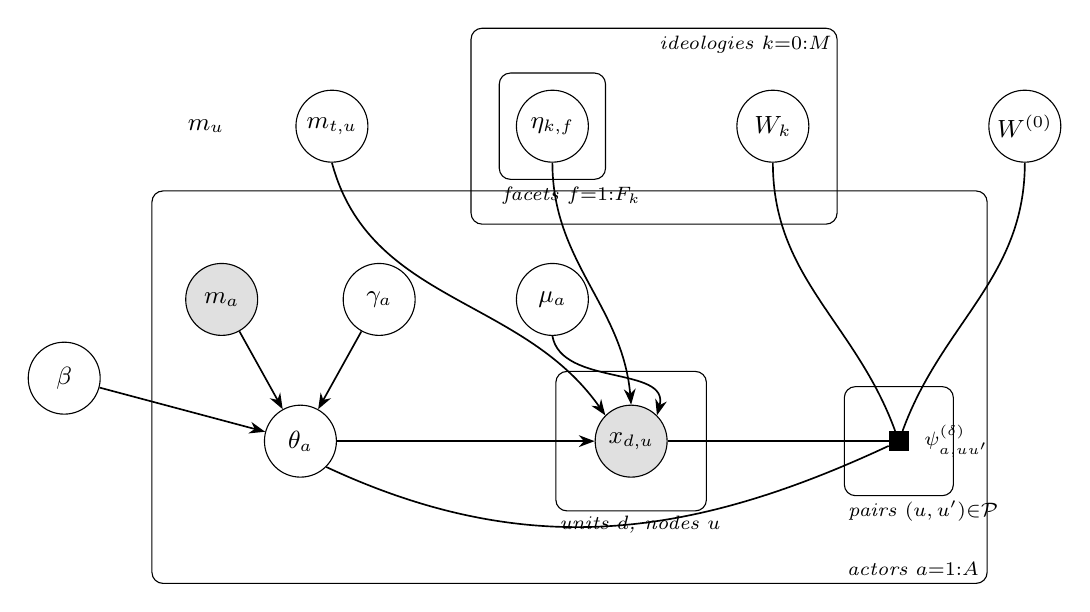
\begin{tikzpicture}[
  latent/.style={draw,circle,minimum size=26pt,inner sep=1pt,font=\small},
  obs/.style={draw,circle,fill=black!12,minimum size=26pt,inner sep=1pt,font=\small},
  factor/.style={draw,fill=black,minimum size=7pt,inner sep=0pt},
  fix/.style={font=\small},
  plate/.style={draw,rounded corners,inner sep=8pt},
  >=Stealth, edge/.style={->,semithick}, fedge/.style={-,semithick}
]
% top row
\node[fix]    (m)  at (0.2,5.4) {$m_u$};
\node[latent] (mt) at (1.8,5.4) {$m_{t,u}$};
\node[latent] (etak) at (4.6,5.4) {$\eta_{k,f}$};
\node[plate,fit={(etak)},inner sep=6pt] (pf) {};
\node[font=\scriptsize\itshape,anchor=north west] at ([xshift=-2pt,yshift=1pt]pf.south west) {facets $f{=}1{:}F_k$};
\node[latent] (Wk)   at (7.4,5.4) {$W_k$};
\node[plate,fit={(pf) (Wk)},inner ysep=16pt,inner xsep=10pt] (pk) {};
\node[font=\scriptsize\itshape,anchor=north east,inner sep=2pt] at ([yshift=-1pt]pk.north east) {ideologies $k{=}0{:}M$};
\node[latent] (W0) at (10.6,5.4) {$W^{(0)}$};
% actor plate
\node[latent] (beta)  at (-1.6,2.2) {$\beta$};
\node[obs]    (ma)    at (0.4,3.2) {$m_a$};
\node[latent] (gam)   at (2.4,3.2) {$\gamma_a$};
\node[latent] (theta) at (1.4,1.4) {$\theta_a$};
\node[latent] (mua)   at (4.6,3.2) {$\mu_a$};
\node[obs] (x) at (5.6,1.4) {$x_{d,u}$};
\node[plate,fit={(x)},inner xsep=14pt,inner ysep=12pt] (pd) {};
\node[font=\scriptsize\itshape,anchor=north west] at ([xshift=-2pt,yshift=2pt]pd.south west) {units $d$, nodes $u$};
\node[factor,label={[font=\scriptsize,xshift=2pt]right:$\psi^{(\delta)}_{a,uu'}$}] (F) at (9.0,1.4) {};
\node[plate,fit={(F)},inner xsep=16pt,inner ysep=16pt] (pp) {};
\node[font=\scriptsize\itshape,anchor=north west] at ([xshift=-2pt,yshift=2pt]pp.south west) {pairs $(u,u'){\in}\PP$};
\node[plate,fit={(ma) (gam) (theta) (mua) (pd) (pp)},inner xsep=12pt,inner ysep=26pt] (pa) {};
\node[font=\scriptsize\itshape,anchor=south east,inner sep=3pt] at (pa.south east) {actors $a{=}1{:}A$};
% directed edges
\draw[edge] (beta) -- (theta);
\draw[edge] (ma) -- (theta);
\draw[edge] (gam) -- (theta);
\draw[edge] (mt.south) to[out=-75,in=125] (x.north west);
\draw[edge] (etak.south) to[out=-90,in=95] (x.north);
\draw[edge] (mua.south) to[out=-80,in=75] (x.north east);
\draw[edge] (theta.east) -- (x.west);
% factor edges
\draw[fedge] (x.east) -- (F);
\draw[fedge] (Wk.south) to[out=-90,in=110] (F);
\draw[fedge] (W0.south) to[out=-90,in=70] (F);
\draw[fedge] (theta.south east) to[out=-25,in=-155] (F);
\end{tikzpicture}
\caption{\small Hybrid diagram: a directed generative rate layer and an undirected estimating factor. Shaded: observed. Membership $\theta_a$ (softmax of ideology logits $\beta^\top m_a$ and facet logits $\gamma_a$, over $(k,f)$ pairs including background $k{=}0$) composes the rate through the facet profiles $\eta_{k,f}$ and routes pair excess through its ideology margin $\vartheta_a$; facets share their ideology's $W_k$. The filled square is the pair-channel estimating function---a factor, not a child: no joint distribution over $(x,A^{(\delta)})$ exists in the model (see \emph{status of the pair channel}). Sparsity scales $\tau^{(I)}$ folded into $\eta_{k,f}$; fixed $m_u$ unboxed.}
\end{figure}

\section{Theory in the model}\label{sec:constraints}

Each item names where it appears in the generative story and its register: priors make claims of degree, caps and zeros make claims of possibility.

\subsection*{C1. Concept--ideology affiliation (prior on $\eta_k$)}
The mean shift $\pm\alpha$ on $\Acal^\pm_k$ in the facet-profile draws, shared by all facets of $k$: affiliation is a property of the ideology, and facets differ in engagement, not allegiance. Theory asserts direction; the data sets magnitude, since the deviation is free around the shifted mean. Affiliations are partial and historically contingent---anchor only definitional cores.

\subsection*{C2. Within-ideology links (prior on $W_k$)}
The shifted support $W_{k,uu'}\ge\omega$ on $\Ecal_k$ in the network draw. $\Ecal_k$ need not agree across ideologies; both $\Ecal_{\text{intersectional}}$ and $\Ecal_{\text{nationalist}}$ can involve \node{race}{central} with different partners.

\subsection*{C3. Incompatibility (cap on $\eta_k$; zeros in $W_k$; inputs)}
Incompatible sets $\mathcal{S}=\{\NN_c\}_{c}\cup\Xcal$: structural sets (the levels of each concept) are incompatible by construction and bind at every layer---inputs (level co-counts within a unit projected if violated), profiles (the cap $\sum_{u\in S}e^{m_u+\eta_{k,f,u}}\le\bar\pi$, \emph{per facet}), networks ($W_{k,uu'}=0$ on same-concept pairs, vacuous under the one-node-per-concept codebook). Theoretical sets $\Xcal$ are incompatible by substantive judgment, are revisable, and bind \emph{only} the ideology layer. The cap binds per facet, and per facet is enough: the composed sum $\sum_{u\in S}e^{m_u+\sum_f\theta_f\eta_{k,f,u}}$ is convex in the membership $\theta$, so its maximum over the facet simplex is attained at a vertex---a single facet---and mixing facets only dilutes (geometric means of elevations). Per-facet caps therefore bound every adherent of $k$, however specialized or mixed within it. What they do not bound is \emph{distributive} incompatibility: the ideology's platform (the union of facet supports) may contain a theoretical set partitioned across facets that no single adherent composes. That is deliberately a diagnostic rather than a constraint---an ideology whose wings hold contradictory positions is the ``facets were ideologies all along'' situation, so any $S\in\Xcal$ intersecting two facets' supports of one $k$ is reported as a split signal alongside the release-the-tie test (Section~\ref{sec:inference}). Cross-ideology mixing can still compose violations: units and actors can be incoherent---ideologies cannot---and a straddler is not an ideology. The gap between layers is reported, not absorbed (Section~\ref{sec:inference}).

\subsection*{C4. Actor alignment (prior on $\theta_a$ via metadata)}
The alignment regression, acting on the ideology margin of the membership: identity informs which ideology, never which facet---facet choice within an ideology is an actor-level draw, so that specialization is not confused with identity. $\beta$ generalizes labeled anchors ($\Tcal^{\text{fix}}$, which pin ideologies to names and break label switching) to unlabeled actors. Inverted, the fitted regression gives each ideology an adherent identity profile---an estimand rather than a definition.

\subsection*{C5. Type ladder (zeros in $W^{(0)}$ and $W_k$)}
$W_{uu'}=0$ off $\PP$, i.e.\ on rung-skipping pairs $\{VB,VR,AR\}$, for the shared layer and every ideology. Intra-type blocks ($V\!-\!V$, $A\!-\!A$, $B\!-\!B$, $R\!-\!R$) are admitted: the ladder forbids skipping, not lateral structure. Consequences: cross-rung paths pass through adjacent rungs, so the middle layers mediate between distant rungs by construction; the ladder is testable---systematic excess pairing on rung-skipping pairs, computed exactly as the $R$ diagnostic but off $\PP$, is evidence against a type assignment, reported per pair. One consequence to watch rather than celebrate: intra-rung blocks, especially $B\!-\!B$, can absorb co-occurrence that previously had to load on cross-rung edges, so fitted cross-rung structure will thin; the sparsity penalty, not the typing, is what keeps lateral blocks from dominating, and per-block edge mass is reported.

\subsection*{C6. Structural coherence (statistic first, prior second)}
The framework requires concepts within an ideology to be structurally and logically coherent: more and/or stronger relations to concepts inside the ideology than outside it. Logical coherence is C3. Structural coherence is a claim about the shape of $W_k$ relative to the ideology's support $S_k=\{u:\max_f\eta_{k,f,u}>0\}$ (the union of its facets' supports), and it is implemented in two stages so it remains falsifiable.
\begin{itemize}
  \item \emph{Statistic.} The coherence ratio
  \[
    C_k \;=\; \frac{\sum_{u,u'\in S_k}W_{k,uu'}}{\sum_{u\in S_k,\,u'\notin S_k}W_{k,uu'}},
  \]
  reported per ideology and per $\delta$, against a permutation null (random supports of matched size and degree structure). A component whose structure leaks across its own boundary is either mis-supported or not an ideology by this framework's definition---a reportable failure, not a fitting error.
  \item \emph{Prior (optional, only after the statistic survives unpenalized).} Support-gated sparsity: boundary pairs pay more,
  \[
    \lambda_{k,uu'} \;=\; \lambda_{\text{out}}-(\lambda_{\text{out}}-\lambda_{\text{in}})\,\sigma(\textstyle\max_f\eta_{k,f,u})\,\sigma(\max_f\eta_{k,f,u'}),\qquad \lambda_{\text{out}}>\lambda_{\text{in}},
  \]
  replacing $\lambda_{\text{sp}}$ in the ideology layers ($W^{(0)}$ keeps the flat penalty: culture owes no coherence to any support). The gate makes edges cheaper where profiles are elevated, so $W$ exerts upward pressure on $\eta$; the rate likelihood disciplines this, and the coupling is named in Section~\ref{sec:watch}. The hard limit $\lambda_{\text{out}}\to\infty$ restricts $W_k$ to $S_k\times S_k$---the estimation floor of earlier versions, re-derived from theory rather than computation.
\end{itemize}

\subsection*{C7. Domain}
Rates positive by construction; $W^{(0)},W_k\ge0$, symmetric; kernel and timescale $\delta$ stated with every reported network.

\section{The objective}\label{sec:objective}

M-estimation over $(\eta,W,\beta,\gamma,\mu)$ with variational treatment of the variances $\tau$: rate likelihood plus pair estimating function plus priors-as-penalties (Section~\ref{sec:generative}, status of the pair channel). Writing $\eta_{a,u,t}$ for the composed rate and $\Omega_{a,uu'}=W^{(0)}_{uu'}+\sum_k\vartheta_{a,k}W_{k,uu'}$, $\vartheta_{a,k}=\sum_f\theta_{a,kf}$:
\begin{align*}
  \Lcal \;=\;
  &\sum_d\sum_u\Big[\eta_{a(d),u,t(d)}-x_{d,u}\log\eta_{a(d),u,t(d)}\Big]
  &&\text{(rates)}\\
  +\;&\sum_a\sum_{(u,u')\in\PP}\Big[N^{(\delta)}_a\eta_{a,u}\eta_{a,u'}e^{\Omega_{a,uu'}}-A^{(\delta)}_{a,uu'}\,\Omega_{a,uu'}\Big]
  &&\text{(pairs at }\delta\text{)}\\
  +\;&\lambda_{\text{sp}}\!\!\sum_{(u,u')\in\PP}\!\!W^{(0)}_{uu'}\;+\;\sum_{k,(u,u')\in\PP}\lambda_{k,uu'}W_{k,uu'}
  \;+\;\text{SAGE priors on }\eta_{k,f}\;+\;\text{Gaussian priors on }\beta,\gamma,\mu,m_{t,c}
  &&\text{(priors)}
\end{align*}
subject to the C3 caps and the C2/C5 support of $W$.

\paragraph{Convexity.} Each block, others fixed: the rate terms are concave in each additive log-rate component ($\eta_{k,f}$, $\mu_a$, $m_{t,c}$---log-link Poisson regression), and the SAGE priors are conditionally Gaussian given $\tau$, with closed-form variational updates for $\tau$. The pair terms are convex in $W$ (Poisson GLM with $\ell_1$); the alignment block is a multinomial logistic regression. Block-coordinate descent applies; every step is a sparse GLM.

\section{Inference and diagnostics}\label{sec:inference}

\begin{enumerate}
  \item \textbf{Membership step.} Posterior over $\theta_a$ (ideology $\times$ facet, plus background) from the regression prior, the facet-logit prior, and the actor's aggregate loss; ideology fixed for $a\in\Tcal^{\text{fix}}$, facets always free. One membership per actor, informed by the whole stream.
  \item \textbf{$\beta$-step.} Ridge multinomial regression of ideology-level memberships $\vartheta_a$ on metadata.
  \item \textbf{$\eta_{k,f}$-step / $\mu$-step / $m_{t,c}$-step.} Sparse log-link Poisson regressions with SAGE variance updates (Newton steps linear in the number of active cells); the optional Laplacian smoothing of facet profiles adds a quadratic term.
  \item \textbf{$W$-step.} A nonnegative $\ell_1$-penalized Poisson GLM on allowed pairs, jointly over $W^{(0)}$ and $\{W_k\}$: kernel-weighted counts as observations, $N^{(\delta)}_a\eta_{a,u}\eta_{a,u'}$ as exposure, $(1,\vartheta_a)$ as design---an intercept (culture) plus alignment covariates (ideologies), which is what makes the culture/ideology split an estimation property rather than a definition.
  \item \textbf{Scale step.} $(\sigma_m,\sigma_\mu,\sigma_\xi,\lambda_{\text{sp}})$ by profile likelihood; $\delta$ swept, not optimized.
\end{enumerate}

\paragraph{Residual diagnostic.} For each $k$ and pair with both profile rates elevated,
\[
  R^{(\delta)}_{k,uu'}=\frac{\sum_a\vartheta_{a,k}\,A^{(\delta)}_{a,uu'}}{\sum_a\vartheta_{a,k}\,N^{(\delta)}_a\,\eta_{a,u}\eta_{a,u'}}.
\]
On allowed pairs, $R>1$ is what $W\ge0$ captures; structured $R<1$ among high-profile pairs is a negative edge the model refused to fit---the signature of sub-tendencies the current facets do not resolve, and the signal to raise $F_k$ or split $k$. The composed $\eta_a$ terms in the denominator prevent facet-level specialization from masquerading as fragmentation. The facet/ideology boundary is itself testable: refit with the tie on $W_k$ released (one network per facet); if the freed networks diverge on well-estimated pairs, the facets were ideologies all along, and the tied fit was undercounting $M$. On rung-skipping pairs, structured $R>1$ is evidence against the ladder or a type assignment, reported per pair. All of it is a function of $\delta$; an edge present at small $\delta$ and absent at large (or the reverse) is a finding about where structure lives, not an inconsistency.

\paragraph{Contestation typology.} Per concept, from the fitted facets: \emph{cultural}---$m$ high, $\eta_{k,\cdot}\approx0$ for all $k$, association only in $W^{(0)}$; \emph{consensually ideological}---one level elevated near-identically across ideologies; \emph{contested by exclusion}---ideologies split on which level is elevated; \emph{contested relationally}---shared elevated node, diverging $W_k$ rows. Reported as the dispersion of $\eta_{k,u}$ across $k$ (presence contestation) and row-wise divergence of $W_k$ at shared nodes (relational contestation). The model-external check of the van Dijk distinction: for cultural nodes, alignment should add no predictive power for expression---if it does, the node is not culture.

\paragraph{Choosing $M$.} Held-out fit plus the split diagnostic. The zero-ideology null permutes actor metadata and shuffles alignments, refitting memberships with breadth $\mu_a$ held at its real-fit value (memberships refitted freely re-absorb the structure the permutation removed). A corpus that does not beat this contains no coherent ideology in the framework's sense.

\paragraph{Incoherence statistics.} For each theoretical set $S\in\Xcal$: the unit-level violation rate $V_S=\frac1D\sum_d\1[\sum_{u\in S}x_{d,u}>1]$, the actor-level rate $V^{\text{actor}}_S=\frac1A\sum_a\1[\sum_{u\in S}\eta_{a,u}>\bar\pi]$, and their decompositions by alignment. Violations concentrated in an actor measure that actor's inconsistency; concentrated in a component, they mean the component is mis-fit or $\Xcal$ is wrong. Additionally, per ideology: the distributive-incompatibility indicator---any $S\in\Xcal$ intersecting the supports of two facets of the same $k$---reported as a split signal (C3), read together with the release-the-tie test above. Every hard constraint on ideologies keeps a soft residual on data.

\section{Why single-graph methods fail on relational contrast}\label{sec:single}

Pool all evidence into one co-occurrence graph and the racial-ideology example produces a correct-edge-by-edge, wrong-as-structure picture: a path \node{racism}{structural}~--~\node{race}{central}~--~\node{hierarchy}{natural} that no actor and no ideology walks, because the two edges into the shared node come from disjoint sets of actors. A method reading structure off the pooled graph must cut the bridge, merge across it, or fall back to rank-one overlapping factors. One edge weight per pair per ideology, with actor excess routed by alignment, is the minimal model that does none of these---and the argument is indifferent to $\delta$: the pooled graph fails at every timescale for the same reason. The shared layer $W^{(0)}$ is not a retreat to the pooled graph: it carries only association common to \emph{all} actors, while the pooled graph's failure is precisely that it merges association specific to disjoint groups.

\section{Positioning}\label{sec:related}

\paragraph{The expression layer is a structural topic model over concepts.} The rate equation is SAGE: a background log-frequency, sparse additive deviations per layer (time, ideology-facet), no switching variables; actors are mixed memberships over sub-profiles rather than carriers of their own deviation layer, which moves the actor side from SAGE toward classic mixed membership, sparsity from a scale-mixture prior. The alignment regression is STM's prevalence covariates, with identity metadata in place of document covariates. Concepts replace words; typed, leveled nodes replace the vocabulary. Setting $W=0$ \emph{is} an STM variant, which is therefore the baseline every edge-related claim must beat. The shared association layer is the intercept of the pair channel, as the background $m$ is of the rate channel; both implement the culture/ideology distinction as shared-versus-alignment-covarying. The departures from that family: (i) the pair channel---topic models have no within-document or within-author interaction term, and $W$ at any $\delta$ is outside them; (ii) levels with exclusion, and the typed ladder---a vocabulary has no mutually exclusive levels of a word; (iii) Poisson rather than multinomial normalization, because units express variable numbers of nodes and absence is informative.

\paragraph{ResIN.} Response-level nodes and the practice of working without negative edges are taken from ResIN, with a different warrant (the remark in Section~\ref{sec:generative} rather than $\phi$-saturation). ResIN's edge weight is a correlation across respondents---the large-$\delta$ endpoint of the channel, computed on complete survey data where every respondent answers every item and absence is never ambiguous. In discourse, absence is apportioned among background, profile, and repertoire, and the small-$\delta$ endpoint has no survey analogue at all, since a survey has one ``unit'' per respondent. ResIN remains the initializer (clusters seed alignment) and the no-relational-contrast baseline.

\paragraph{BENDING.} The participant-by-item co-endorsement projection is the pooled between-actor graph: the large-$\delta$ endpoint with communities given and one component per community. The model generalizes it by inferring alignment through identity metadata---making ``bears on the community's identity'' an estimand---and by letting a node sit in several components with different neighborhoods. Idiosyncrasy is still not centrality: \node{race}{central} fails BENDING's idiosyncrasy while being the hub of two structures; sharedness, distinctiveness, and structural centrality ($\eta_{k,u}$, $\eta_{k,u}-\max_{k'\ne k}\eta_{k',u}$, $\sum_{u'}W_{k,uu'}$ within type) remain the repair. The Macy et al.\ ``worlds'' result remains the reason C1 anchors only definitional cores.

\paragraph{Networks of Beliefs.} $(\eta_k,W_k)$ are local fields and couplings, per ideology; the remark makes NB's signed couplings over concepts and unsigned $W$ over levels the same family, conditional on expression. NB supplies the reason discrete ideologies exist (low-attention unimodality vs.\ high-attention multimodality of the coupled landscape); the zero-ideology null is the high-temperature regime, and the all-zeros deviation is its resting place. The actor-level analogue of NB's personal temperature is the background share $\theta_{a,0}$ and the entropy of the ideology margin $\vartheta_a$---how far an actor sits from every attractor. NB's couplings connect any pair; C5 asserts they skip no rungs, and NB could absorb that as a sparsity pattern; C6's coherence ratio has an NB reading too---an attractor whose couplings mostly leave its own support is a shallow basin. What NB has that this model lacks: dynamics, social beliefs as a node class, the network of others' actual beliefs; running NB's dynamics on a fitted $(\eta_k,W_k)$ landscape is the natural extension.

\section{Build order, and what each facet is for}\label{sec:build}

The additive layers are not interchangeable regressors: each exists to protect the interpretation of the ones after it, and several layers compete for the same variance. The build order is therefore a sequence of \emph{attribution contests}, each stage asking whether the next layer claims variance the previous ones were holding---and dropping a layer is not a simplification but a reattribution, whose destination should be known in advance.

\begin{enumerate}
  \item \textbf{Single-facet rates.} Background $+$ one profile per ideology ($F_k=1$), membership from metadata plus the background coordinate, $W=0$. Tests whether anchors and metadata are consistent with the data; the background coordinate $\theta_{a,0}$ gives off-profile chatter a home, so this stage already degrades gracefully for mildly off-profile actors.
  \item \textbf{Facets.} Raise $F_k$, selected by whole-actor holdout (V7). This is the specialist stage: without facets, a single-issue account's silence on the rest of its ideology's platform counts as evidence against its alignment, pushing specialists toward background or minting junk components; with them, the silence is the facet's. Report the specialist tail---per-actor held-out fit at $F_k=1$---as the direct measure of how much this stage was needed. The withheld-concept test (V5) runs here: the prediction is facet-composed, $\sum_{k,f}\theta_{a,kf}\eta_{k,f,u}$.
  \item \textbf{The pair channel at $\delta=0$, shared layer first.} Add $W^{(0)}$ alone, then $\{W_k\}$; movement between the two fits is the association mass that is genuinely ideological. Run the $R$ diagnostic on allowed and rung-skipping pairs, and the coherence ratios (gate off).
  \item \textbf{Temporal background, then sweep $\delta$.} $m_{t,c}$ enters here, not earlier: it is the one facet with no theoretical content, existing purely to protect the others' interpretation, and what it protects is $\delta>0$. Without it, event-driven co-surges are quadratic in the pair counts: a uniform surge is absorbed by $W^{(0)}$ (silently redefining culture to include the news), and a camp-differential surge---event exposure correlated with alignment---is written into $W_k$ as an edge that was merely co-topical for a week. Report the sensitivity of $W(\delta)$ to the temporal resolution of $m_{t,c}$; dropping $m_{t,c}$ is defensible only for short corpora or $\delta\approx0$ questions, and must be paired with the redefinition of $W^{(0)}$ stated aloud. Then sweep: $W_k(\delta)$ as a curve locates the timescale of each edge.
  \item \textbf{Theoretical sets $\Xcal$}, tracking incoherence statistics at all layers.
\end{enumerate}
Stages 1--3 are one warm-started fit. Report the stage at which held-out fit stops improving; that is itself a finding about how much coherence the discourse exhibits and where it lives.

\paragraph{The facet--$W$ contest.} The fundamental attribution contest of earlier versions---free actor deviations $\varepsilon$ versus $W$ as rival explanations of between-actor covariation at large $\delta$---is resolved by design: actor variation is rank-restricted to the facet span, so covariation beyond the facets must land in $W$, and no per-actor shrinkage scale couples to the edges. But the contest re-enters through the facet count: each added facet is a rank of between-actor covariation that $W$ no longer has to explain, and at $F_k$ large enough the facets \emph{are} free deviations again. The dial is now discrete, selected by whole-actor holdout rather than tuned continuously, which is the point---but the required report survives in new form: $W_k$ at large $\delta$ across the $F_k$ ladder. Stable $W$ as facets enter means edges and specialization carry different variance; $W$ collapsing into new facets means ``ideological structure'' and ``specialist composition of adherents'' are the same variance under two names, a limitation to state, not to tune away. The old free-$\varepsilon$ model remains the saturated endpoint of this ladder, fit once as an upper bound, not a candidate.

\section{Things to watch}\label{sec:watch}

\paragraph{Identifiability.} Actor deviations and ideology profiles trade off: a facet with a single high-membership actor cannot be separated from that actor's idiolect; report effective actors per facet and read single-actor facets as that actor's version of the ideology. At the large-$\delta$ endpoint, $W$ and the facet count are coupled; the facet--$W$ contest of Section~\ref{sec:build} is the required report.

\paragraph{Mixing actors.} Soft membership carries straddlers; per-actor entropy over the \emph{ideology} margin $\vartheta_a$ (not facets---facet spread within an ideology is specialization, not mixing) is the surveillance instrument, and a cluster of high-entropy actors between two components is evidence for a missing component or a bridging tendency worth naming.

\paragraph{The coherence gate.} If the C6 prior is switched on, edges are cheaper where profiles are elevated, so the pair channel pushes $\eta$ upward at nodes it wants to connect; report fits with the gate on and off, and treat divergence between them as the gate speaking rather than the data.

\paragraph{Lateral absorption.} Intra-rung blocks (especially $B\!-\!B$) compete with cross-rung edges for the same co-occurrence; per-block edge mass and the sensitivity of cross-rung structure to the lateral blocks' penalty are reported.

\paragraph{The news cycle.} $m_{t,c}$ absorbs shared topical shocks so they are not read as edges; it competes with $W$ at moderate $\delta$ (an event drives one camp to pair two concepts for a week). Sensitivity of $W(\delta)$ to the temporal resolution of $m_{t,c}$ is reported.

\paragraph{Type assignments.} A concept mistyped one rung off shows up as rung-skipping excess with its true neighbors, at whatever $\delta$ its links live; treat the residual as a prompt to revisit $T(c)$ before the ladder.

\paragraph{Extraction noise.} A per-concept miss rate is confounded with the additive intercepts (an under-detected concept looks like a low-rate one); it is invisible to the corpus alone and enters as a fixed offset once calibration against hand-coded units pins it. Multiplicative recall cancels in $W$ (pair counts and exposure scale together), so the association layer is robust to the error type least identifiable from residuals.

\paragraph{Expressed vs.\ held.} The model measures expressed ideology; the rationalization rung carries the largest share of the expression--belief gap, and the $\delta$-dependence of $B\!-\!R$ edges (present within expressions, absent in dispositions, or the reverse) is a partial instrument for it.


\section{Extensions (not implemented)}\label{sec:extensions}

\paragraph{A coherent generative pair model.}

The estimating-equation status of the pair channel is a choice, not a necessity. The coherent alternative generates dependence in $x$ directly, by \emph{common shocks}: for each actor and pair $(u,u')\in\PP$, a latent stream of co-activation events
\[
  Z_{a,uu'} \sim \text{Poisson process, rate} \propto \eta_{a,u}\,\eta_{a,u'}\big(e^{\Omega_{a,uu'}}-1\big),
\]
each event depositing one count on $u$ and one on $u'$ at a temporal separation drawn from a footprint distribution with scale $\delta$; observed expression is idiosyncratic counts plus shocks. Then $x$ is the only observed object, $A^{(\delta)}$ is demoted from pseudo-observation to sufficient-statistic summary computed in inference, pair counts carry excess $e^{\Omega}$ in expectation---and $\delta$ is promoted from analyst kernel to \emph{estimand}: the temporal footprint of a coherent episode, how long an ideological co-activation lasts in an actor's stream. Costs, priced: marginal rates inflate by the shock mass, so the rate facets need centering for $\eta$ to keep its meaning; and inference moves from two sparse GLMs to EM over latent shock attributions (multivariate Poisson factorization---each step tractable, the whole materially heavier). The estimating-equation model of Section~\ref{sec:generative} is the working version; this is its principled successor, and the reinterpretation of $\delta$ is the reason to eventually pay for it. Beyond it, two further extensions. \emph{Seeded diffusion}: replace facets by engagement generated from the network itself---sparse seed concepts $s_a$ spreading along the ideology's edges, engagement $\propto(I-\beta_d\Wt_{k})^{-1}s_a$---so a specialist is ``seeded at redistribution, decaying along ladder paths,'' repertoire boundaries inform $W$ through the rate likelihood, and the claim that specialties respect edge structure becomes falsifiable (focal sets straddling disconnected regions of $W_k$ refute it); the cost is coupling $W$ into the rate channel. And the earlier ones stand: NB dynamics on a fitted $(\eta_k,W_k)$ landscape, and drift in profiles over long horizons.
\paragraph{Prediction-powered inference for the extractor.} The extractor's $\hat x$ stands in for true expression everywhere; a hand-coded gold set $\mathcal{G}$ could correct for this without any model of extractor error, by rectifying the estimating equations themselves. With $\psi(\cdot;\Theta)$ the stacked score (rate and pair blocks), solve
\[
  \sum_d \psi(\hat x_d;\Theta)\;+\;\frac{D}{|\mathcal{G}|}\sum_{d\in\mathcal{G}}\big[\psi(x^*_d;\Theta)-\psi(\hat x_d;\Theta)\big]\;=\;0,
\]
where the second term---the rectifier---is the estimated bias of the extractor-scored gradient at the current parameters. Gold data then informs how the model \emph{interprets} predictions rather than relabeling them: all estimands ($\eta_{k,f}$, $W$, coherence ratios, contestation and incoherence statistics) inherit the correction, with confidence intervals merging into the sandwich errors the composite likelihood already requires. Four consequences worth recording now, since they constrain design before any implementation. (i) The pair-block rectifier is the valuable one: it corrects correlated co-attribution---the extractor reading one theme and depositing several nodes---so rectified-versus-unrectified $W$ separates extractor-robust edges from artifacts, superseding the $\delta{=}0$-versus-$\delta{>}0$ heuristic; intra-rung blocks, where co-attribution of topically adjacent concepts is worst, would be disciplined first. (ii) The kernel dictates the coding design: rectifying cross-unit scores at lag $\delta$ requires \emph{gold pairs}---contiguous hand-coded runs within an actor's stream---not scattered random units; $W(\delta)$ is rectifiable only at timescales the gold-pair design covers. (iii) Differential extractor error (stance and negation failures concentrate on counter-attitudinal content) is handled by stratifying the rectifier, and the theory-driven improbable-extraction flag, unusable as a correction (it would purge the priors' counterevidence), is safe as a \emph{sampling design}: oversample flagged cells with known inclusion probabilities and weight the rectifier accordingly---priors may point the coder, never the corrector. (iv) A power-tuning interpolation per score block would let the data conclude, e.g., that the extractor is reliable for rates but not for pairs. Gold data thus enters three times---bias correction at the score level, variance, and design---and never as per-unit relabeling.

\section{Validation}\label{sec:validation}

Constraints and priors are inputs; each test withholds one and asks whether the model recovers it. The ladder is not held out---its forbidden-pair residuals remain diagnostics of type assignments. Every test reports a baseline. All numbers \textbf{TBD}; results from previous versions' corpus and model are superseded.

\subsection*{V1. Concept--ideology affiliation (C1)}
Drop 30\% of $\Acal^+_k$, refit, rank held-out affiliations against never-affiliated nodes by fitted $\max_f\eta_{k,f,u}$. \textbf{TBD.}

\subsection*{V2. Does supplied theory buy predictive capacity? (C1, C2)}
Supply fractions of $\Acal^+_k$ or $\Ecal_k$; read held-out fit. The prior form removes the magnitude claim that damaged fit before, so the sharp prediction is a flat-to-improving affiliation curve; monotone degradation would now indict the prior means themselves. \textbf{TBD.}

\subsection*{V3. Incompatibility (C3)}
Drop half of $\Xcal$, refit, report $\max_k\sum_{u\in S}e^{m_u+\eta_{k,u}}$ per dropped set against the cap. \textbf{TBD.}

\subsection*{V4. Actor groups}
Posterior alignment against group labels withheld from $m_a$ (ARI and the group-by-component table); the question is which groups the model declines to separate, and whether groups sharing an ideology separate at the facet level---sub-tendency without a further component. \textbf{TBD.}

\subsection*{V5. Actor stance on a withheld concept}
Mask (actor, concept) cells from the rate likelihood; predict the actor's rate as the facet-composed $\sum_{k,f}\theta_{a,kf}\eta_{k,f,u}$ (times breadth and background). Baselines: node rate; breadth $\times$ node rate; peer mean within group label; the $F_k=1$ model. Beating the third is the headline test of the hierarchy; beating the fourth is the facets earning their place. \textbf{TBD.}

\subsection*{V6. The timescale curve}
$W_k(\delta)$ across the sweep, with held-out fit and the $R$ diagnostic at each $\delta$: which edges live within expressions, which in episodes, which in dispositions; whether the theory links $\Ecal_k$ concentrate at a timescale; at the large-$\delta$ end, $W_k$ across the $F_k$ ladder (the facet--$W$ contest of Section~\ref{sec:build}). \textbf{TBD.}

\subsection*{V7. Whole-actor holdout}
Hold out entire actors; score their units with $(\gamma_a,\mu_a)$ marginalized under the prior and the ideology margin from metadata alone. The primary predictive criterion, and the selector of the facet counts $F_k$. \textbf{TBD.}

\subsection*{V8. Structural coherence and the culture/ideology partition (C6, $W^{(0)}$)}
Three readings. (i) Coherence ratios $C_k$ against the permutation null, per ideology and per $\delta$, fitted \emph{without} the gate---the falsifiable form of the coherence requirement. (ii) The share of total edge mass in $W^{(0)}$ versus $\{W_k\}$, and the contestation typology's concept counts: how much of the discourse is culture, how much contested. (iii) The van Dijk check: predictive gain from alignment, per concept; concepts the typology calls cultural should show none. \textbf{TBD.}

\section{Experimental design}\label{sec:experiments}

Section~\ref{sec:validation} lists what the model's inputs owe the data. This section
states the four analyses built \emph{on} those tests, aimed at whether the framework is
useful rather than at whether any single constraint survives being withheld. Each names its
corpus, its fitted configuration, and the confounds the design controls; all numerical
results are \textbf{TBD}.

\paragraph{Corpus and supervision.} The corpus is one snapshot, frozen before the analyses
run and fingerprinted (coding hash, unit and actor counts) in every output, because the
extraction was still being written while the design was fixed: a sweep whose arms are fit on
different snapshots compares nothing. Supervision is three pinned actors per ideology (C4),
chosen by hand:

\begin{center}
\begin{tabular}{@{}llr@{}}
\toprule
ideology & pinned actors & units behind them \\
\midrule
CB & RealCandaceO, bluelivesmtr, PrisonPlanet & 1,718 \\
WS & PatVPeters, BlissTabitha, winstonCovfefe & 73 \\
IS & BreeNewsome, deray, jemelehill & 6,653 \\
\bottomrule
\end{tabular}
\end{center}

\noindent The counts are the first result rather than a footnote. WS's three pins carry 73
units against IS's 6,653, a ratio of 91:1, and one of them carries five. Pinning still does
what C4 exists for---it fixes the correspondence between a component and a name, without
which the components relabel themselves between fits---but three actors and 73 units cannot
\emph{estimate} a profile. So WS is confined to E4, where whether it is a component at all
is the question under test, and every WS quantity is reported beside its effective-actor
count and the units behind its pins. E1--E3 fit $M=2$ (CB and IS), on the reasoning that
concept rankings and centralities drawn from a component we have grounds to doubt would not
mean what they appear to.

\paragraph{Withholding identity.} E1 and E2 fit with the alignment design reduced to an
intercept, so that the metadata carries no information about the actor. Without this both
analyses are circular: E1 scores how well the fitted membership recovers an actor's
community, which is trivial if that community is a column of $m_a$; E2 asks what the pins
alone recover, which is unanswerable if identity is doing the work.

\subsection*{E1. Community identity and the ladder}
Two claims, kept apart because they are different kinds of statement. \emph{Face validity}:
inverted, $\beta$ gives each ideology an adherent identity profile, which is the estimand
C4 promises rather than a definition---read from a fit with the metadata design intact,
since $\beta$ is otherwise empty. \emph{Prediction}: from the intercept-only fits, how well
the ideology margin $\vartheta_a$ recovers community, scored both as an adjusted Rand index
against the hard assignment and as leave-one-actor-out multinomial accuracy---the second
because a Rand index conflates recovery with the number of clusters.

The substantive question is whether using more of the ladder predicts community better, and
the confound is that the rungs are of unequal size ($|V|=13$, $|A|=28$, $|B|=35$, $|R|=36$).
A raw comparison cannot separate ``beliefs carry identity'' from ``beliefs is the larger
rung.'' Three arms therefore hold size fixed: single rungs each sampled down to $|V|=13$
nodes; the cumulative ladders $V$, $V{+}A$, $V{+}A{+}B$, all four; and, at each cumulative
size, a control drawn at random from the whole codebook. Sampling is stratified on C1
anchoring so that node count \emph{and} the amount of supplied theory are matched and only
rung identity varies---feasible because every rung can supply the $V$ rung's exact anchor
profile. The random control is what makes the result readable: without it, a cumulative arm
beating a single rung is uninterpretable, and with it the claim becomes that typed ladder
structure beats an arbitrary subset of equal size and equal supervision.

\subsection*{E2. What pinned actors alone recover}
An analyst adopting this framework can label a few accounts and little else. E2 asks what
that buys. Against a reference fit with the full metadata design, the pin ladder refits with
one, two and three pins per ideology and an intercept-only design, and reports agreement
with the reference on the profiles ($\eta$, by rank and by the overlap of each ideology's
strongest concepts), on the association layer ($W$, over pairs either fit calls live), and
on the actor assignments. Whole-actor holdout (V7) runs alongside as an absolute anchor, so
the curve is not purely relative. Pins are added in order of the units behind them, so the
one-pin arm is the best-evidenced single actor---the realistic case rather than the average
one. The descriptive half of the question, which concepts, actors and edges each ideology is
built from, is read off the reference fit: sharedness, distinctiveness and within-type
centrality per node; edge mass per type block; and the disposition of each theory-supplied
link (confirmed, absorbed into the shared layer, or inert in both).

\subsection*{E3. Targets worth examining}
Four scores per concept per ideology: within-support centrality $\sum_{u'\in S_k}W_{k,uu'}$;
boundary mass $\sum_{u'\notin S_k}W_{k,uu'}$, which is the per-node decomposition of C6's
ratio and so is provably the same quantity C6 reports in aggregate; position on the ladder,
since values ground attitudes and attitudes ground beliefs, making a value upstream of what
it supports; and relational contestation, a concept both ideologies elevate whose $W$ rows
diverge. The quadrant of interest is high centrality with high boundary mass: the bridges
C6 penalises, where an ideology's structure is most exposed.

These are targets worth examining and nothing stronger. The model is observational
co-occurrence read at a chosen timescale; it carries no causal warrant, and the route to one
(Section~\ref{sec:extensions}, running belief dynamics on a fitted landscape) is not
implemented. A concept scoring high here is one whose removal would restructure the fitted
\emph{description}---a hypothesis about intervention, not a prediction of its effect.

\subsection*{E4. How many ideologies}
A ladder of configurations: $W=0$, which is the structural-topic-model variant
Section~\ref{sec:related} names as the baseline every edge-related claim must beat; $M=1$, a
single pooled network, which is the arrangement Section~\ref{sec:single} argues cannot
represent relational contrast; $M=2$ (CB, IS); $M=3$ with WS restored and pinned; and $M=3$
plus one, two and three unanchored components, which is how ``are there more?'' is asked.

Four scoring axes, because held-out fit alone is not a finding about $M$
(Section~\ref{sec:inference}): whole-actor holdout, the primary criterion; held-out units,
secondary; the coherence ratio per component against its permutation null, where falling
below the null is a reportable failure rather than a fitting error; and the split signal,
structured $R<1$ among a component's own elevated pairs. The ablation reports not only what
each component's removal costs but where its adherents go, which is the quantity that
distinguishes a third position from a sub-tendency of an existing one. Restoring WS with a
pin is the fair form of this test: in earlier fits WS had no pinned actor at all, so its
instability was as likely to be the absence of an anchor as the absence of adherents.

\vfill
\noindent\footnotesize
Carpentras D, Lueders A, Quayle M (2024). Response Item Network (ResIN): A network-based approach to explore attitude systems. \emph{Humanities and Social Sciences Communications} 11:589.\\
Vlasceanu M, Dyckovsky AM, Coman A (2024). A network approach to investigate the dynamics of individual and collective beliefs: Advances and applications of the BENDING model. \emph{Perspectives in Psychological Science} 19(2):444--453.\\
Dalege J, Galesic M, Olsson H (2024). Networks of beliefs: An integrative theory of individual- and social-level belief dynamics. \emph{Psychological Review}, advance online publication.\\
van Dijk TA (1998). \emph{Ideology: A Multidisciplinary Approach}. Sage.\\
Angelopoulos AN, Bates S, Fannjiang C, Jordan MI, Zrnic T (2023). Prediction-powered inference. \emph{Science} 382(6671):669--674.\\
Eisenstein J, Ahmed A, Xing EP (2011). Sparse additive generative models of text. \emph{Proceedings of ICML}.\\
Roberts ME, Stewart BM, Airoldi EM (2016). A model of text for experimentation in the social sciences. \emph{JASA} 111(515):988--1003.
\normalsize

\end{document}
